\chapter{Die Analyse und Tests}
\label{cha:Analyse}
Dieses Kapitel beschäftigt sich mit der Analyse der Implementierung und dessen Tests. Es gibt zwei Arten von Tests die implementiert wurden
\begin{itemize}
	\item die \emph{JUnit}-Tests sind die Tests, die nicht auf eine \emph{CDI}-Umgebung angewiesen sind und 
	\item die \emph{CDI-JUnit}-Tests sind die Tests, die auf eine \emph{CDI}-Umgebung angewiesen sind.
\end{itemize}

\section{Die Tests}
Dieser Abschnitt beschäftigt sich mit den Implementieren Tests des Vorlagenmanagements und der Implementierten Konfiguration für die Tests. Für die Tests wurden folgende Bibliotheken verwendet.
\begin{itemize}
	\item\emph{JUnit4} ist ein \emph{Framework}, mit dem wiederholbare Tests implementiert werden können und ist als Standard für Tests in \emph{Java} anzusehen.
	\item\emph{Deltaspike} ist ein \emph{Open-Source}-Projekt der \emph{Apache Software Foundation (ASF)}, die portable \emph{CDI}-Erweiterungen in Form von Modulen bereitstellt und auch eine Erweiterung für \emph{JUnit}-Tests bereitstellt, mit denen Tests in einer \emph{CDI}-Umgebung lauffähig sind.
\end{itemize}
\ \newline
Alle implementierten Tests sind nicht auf einen Anwendungsserver angewiesen und sind innerhalb des lokalen Klassenpfades lauffähig und können daher in jeder Entwicklungsumgebung und bei einem Kompilieren über das \emph{Buildtool Maven} ausführbar.
\newline
\newline
Die Tests wurden wie folgt organisiert.
\begin{itemize}
	\item\emph{com.clevercure.mailing.test.*} 
	\newline
	ist das \emph{Java}-Paket in dem alle implementierten Tests liegen. 
	\item\emph{*.[toTestClass]Tests}
	\newline
	ist das \emph{Java}-Paket, für eine zu testende Klasse, wobei der Paketname den Namen der zu testenden Klasse mit dem Suffix Tests enthält.
	\item\emph{[toTestMethod]Test.java}
	\newline
	ist die implementierte Testklasse für die Tests einer Methode der zu testenden Klasse.
	\item\emph{test\_case}
	\newline
	ist der Name der einzelnen Testmethoden, der wiedergibt was an einer Methode getestet wird. 
\end{itemize}
\ \newline
Die vorgestellte Konvention der Tests wurde so umgesetzt sofern es möglich war. 

\subsection{Die Tests der \emph{CDI}-Erweiterung}
Die Tests aus Abbildung \ref{fig:tests-template-cdi} testen die Implementierungen des Artefakts \emph{mailing-moule-template-cdi} wie
\begin{itemize}
	\item den Klasse \emph{TemplateCdiExtension},
	\item die Klasse \emph{CdiTemplateUtils} und
	\item die Klasse \emph{TemplateResourceProducer}.
\end{itemize}
\begin{figure}[h]
\centering
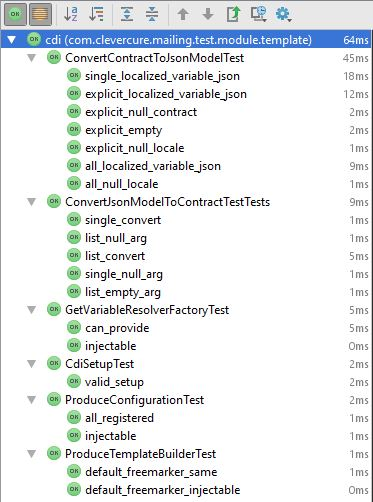
\includegraphics[scale=0.8]{tests-template-cdi}
\caption{Testdurchlauf der Tests der \emph{CDI}-Erweiterung}
\label{fig:tests-template-cdi}
\end{figure}
\ \newpage

\subsection{Die Tests der \emph{Web}-Oberfläche}


\section{Die erreichten Ziele}

\subsection{Das Vorlagen-\emph{Management über \emph{CKEditor}}}

\subsection{Das Vorlagen-\emph{Management} in einer \emph{CDI}-Umgebung}

\subsection{Das Vorlagen-\emph{Management} in JSF}
\subsection{Das Vorlagen-\emph{Management} in \emph{Mail}-DB-Schema}

